% !TeX root = ../Book3.tex
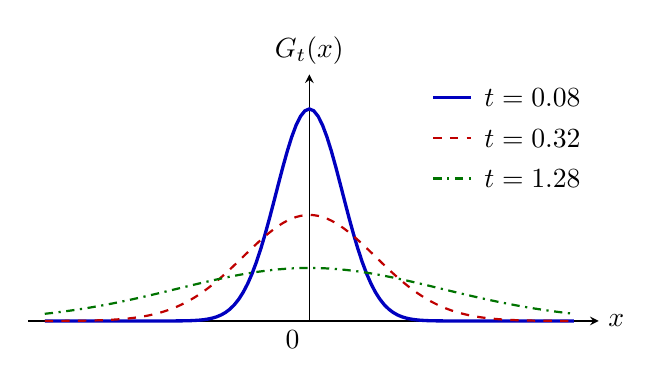
\begin{tikzpicture}[x=1.05cm,y=2.7cm,>=stealth]
	\draw[->] (-3.4,0)--(3.5,0) node[right] {\(x\)};
	\draw[->] (0,0)--(0,1.16) node[above] {\(G_t(x)\)};
	\draw[very thick,blue!75!black,domain=-3.2:3.2,samples=121]
		plot (\x,{exp(-\x*\x/.32)/sqrt(4*pi*.08)});
	\draw[thick,red!75!black,dashed,domain=-3.2:3.2,samples=121]
		plot (\x,{exp(-\x*\x/1.28)/sqrt(4*pi*.32)});
	\draw[thick,green!45!black,dash dot,domain=-3.2:3.2,samples=121]
		plot (\x,{exp(-\x*\x/5.12)/sqrt(4*pi*1.28)});
	\draw[very thick,blue!75!black] (1.5,1.05)--(1.95,1.05);
	\node[right] at (2,1.05) {\(t=0.08\)};
	\draw[thick,red!75!black,dashed] (1.5,.86)--(1.95,.86);
	\node[right] at (2,.86) {\(t=0.32\)};
	\draw[thick,green!45!black,dash dot] (1.5,.67)--(1.95,.67);
	\node[right] at (2,.67) {\(t=1.28\)};
	\node[below left] at (0,0) {\(0\)};
\end{tikzpicture}
